\section{System Implementation (시스템 구현 및 대시보드 시각화)}

제 3장에서 설계한 이론적 아키텍처와 추론 파이프라인을 실제 구동 가능한 프로덕션 레벨의 소프트웨어로 구현하기 위해, 본 프로젝트는 클라우드 기반의 분산 아키텍처와 실시간 시각화가 가능한 프론트엔드 대시보드를 결합하였습니다. 본 장에서는 백엔드 인프라의 최적화 전략과, 블랙박스 AI를 투명하게 공개하는 교육용 `Glass-box' 대시보드의 구현 상세를 다룹니다.

\subsection{클라우드 인프라 및 마이크로서비스 아키텍처 (Backend)}

\subsubsection{모델 런타임 및 하드웨어 추상화}
OMI 파이프라인은 단일 모델에 종속되지 않고 유연하게 동작할 수 있도록 설계되었습니다. 
\begin{itemize}
    \item \textbf{Vertex AI (Gemini) 연동:} 막대한 컴퓨팅 파워와 신속한 추론 속도가 요구될 때, Google Cloud의 Vertex AI 엔드포인트를 호출하여 Gemini 모델 라인업을 사용할 수 있습니다. 이를 통해 복잡한 멀티 에이전트 토론이 요구되는 100회 이상의 호출을 병렬로 처리합니다.
    \item \textbf{로컬/오픈소스 모델 (Qwen 2.5-Math):} CPU Only 환경이나 제한된 GPU 환경을 위한 하드웨어 추상화 계층을 구현했습니다. 환경 변수 \texttt{OMI\_QUANTIZATION=none} 설정 시 CPU에서 경량 모델(1.5B)을 실행하며, GPU 환경에서는 \texttt{vLLM}과 4-bit/8-bit 양자화 기법을 적용해 7B 이상의 수학 특화 모델을 구동합니다.
\end{itemize}

\subsubsection{API 게이트웨이 및 자원 최적화 (Resource Optimization)}
5-Stage 파이프라인은 수많은 백그라운드 추론 호출(API Call)을 발생시킵니다. 특히 다수결 투표(Majority Voting)와 검증 과정을 거치면 단일 문제당 수십 번의 모델 쿼리가 발생하여 클라우드 서비스의 Rate-limit(HTTP 429 Error)에 직면하게 됩니다.
이를 해결하기 위해 우리는 \textbf{Capacity + Token 효율화 실행 계획}을 도입했습니다.
\begin{itemize}
    \item \textbf{리전 다변화 (Region Optimization):} 과부하가 걸리는 \texttt{us-central1} 리전 대신 대기 시간이 짧고 할당량이 넉넉한 \texttt{us-east5} 리전 등으로 엔드포인트를 분산하여 Throughput을 극대화했습니다.
    \item \textbf{동적 타임아웃 및 폴백(Fallback):} 샌드박스에서 파이썬 코드가 무한 루프에 빠지는 것을 방지하기 위해, \texttt{OMI\_EXECUTOR\_TIMEOUT}을 동적으로 조절하여 5초 이상 연산이 지연될 경우 즉각 프로세스를 킬(Kill)하고 모델에게 시간 초과 피드백을 전달합니다.
\end{itemize}
이러한 클라우드 API 최적화 계획과 Throughput 분산 및 자원 관리의 통계적 우수성은 대시보드의 "Comparison" 페이지를 통해 실시간으로 집계 및 시각화됩니다. 그림 \ref{fig:dashboard_comparison}는 GPT-4o 단일 베이스라인 대비 본 연구에서 제안한 OMI 오케스트레이터 파이프라인의 전반적인 정확도(Accuracy) 및 비용 효율성 향상 지표를 직관적으로 비교하고 있습니다.

\begin{figure}[htbp]
\centering
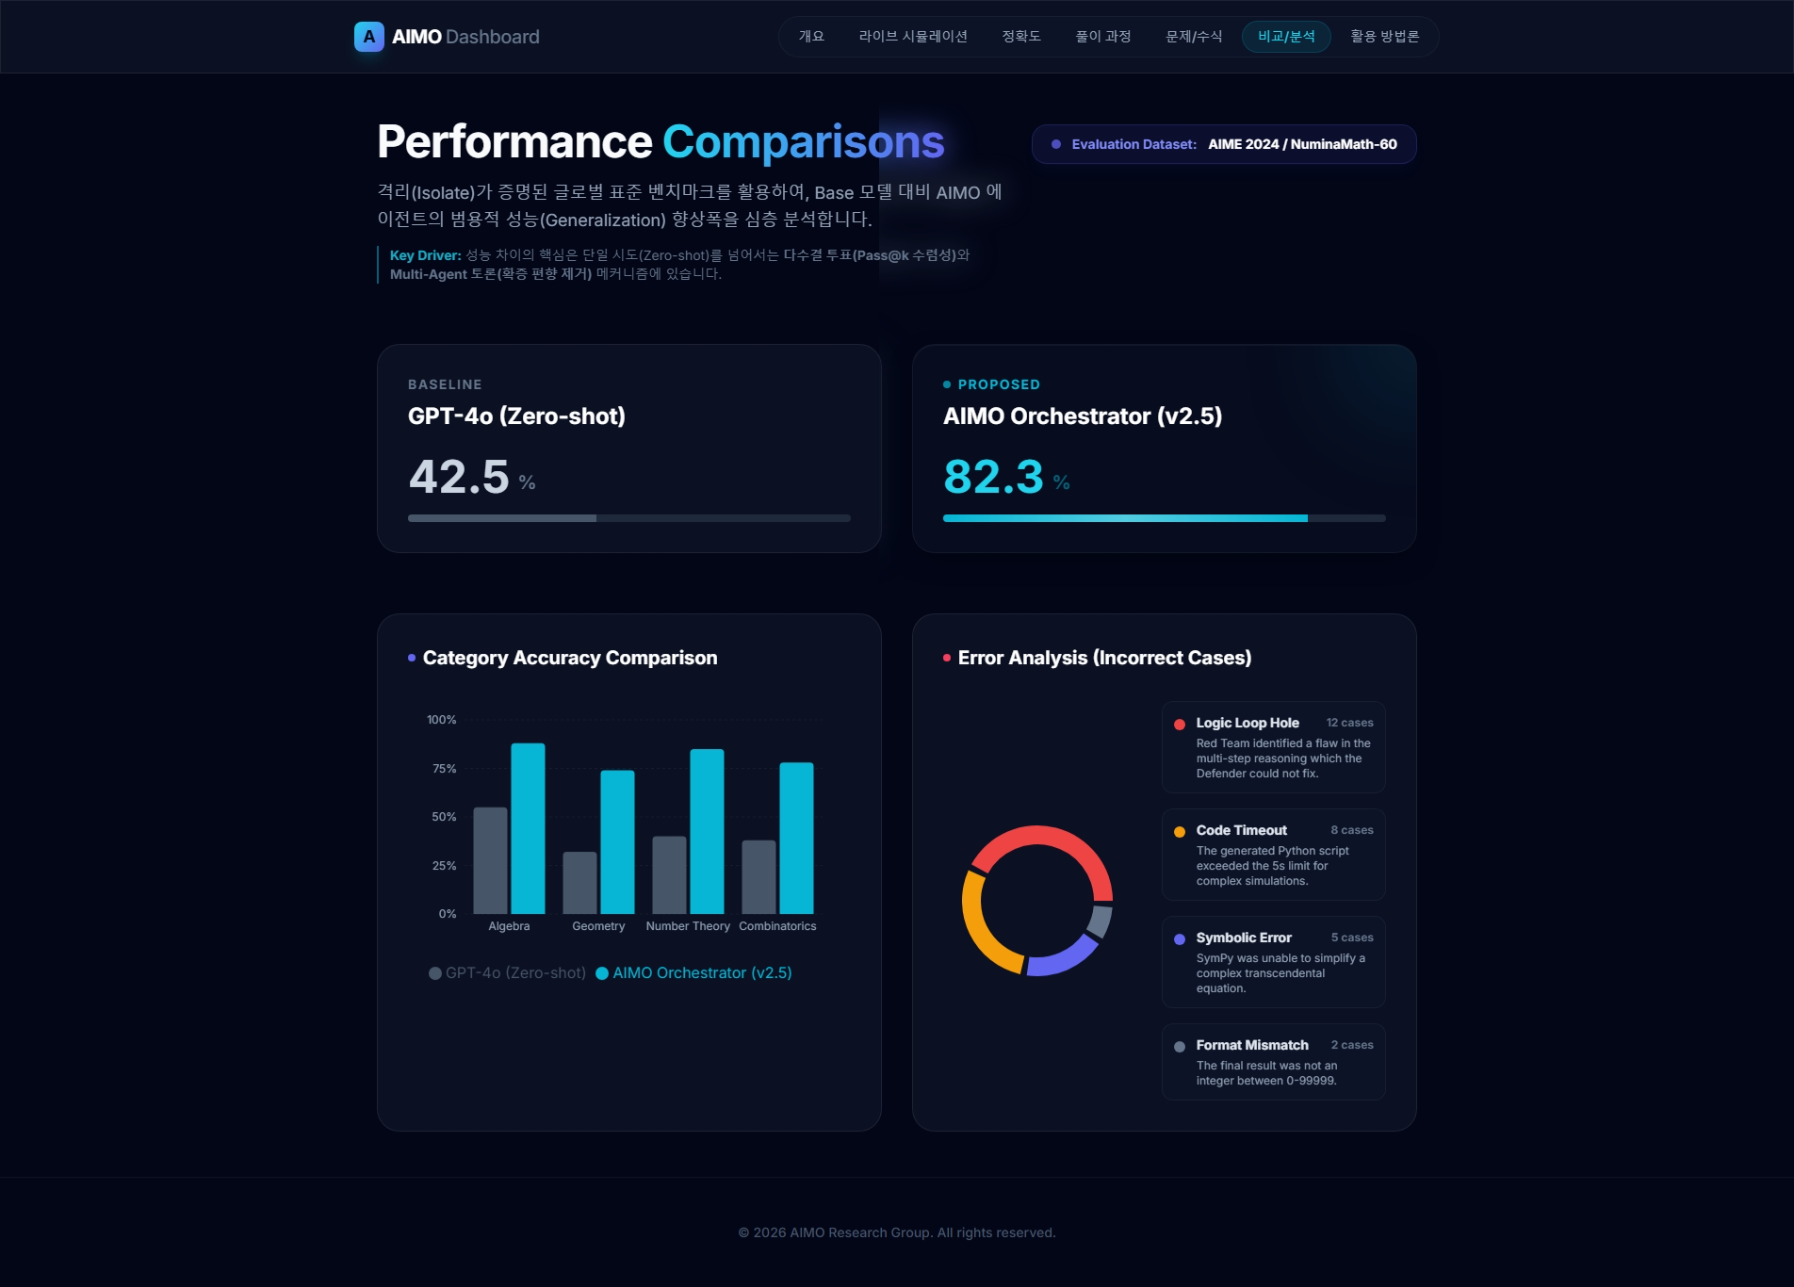
\includegraphics[width=0.95\textwidth]{dashboard_comparison.png}
\caption{Proposed OMI 오케스트레이터 파이프라인과 GPT-4o 베이스라인 간의 최종 수학 해결 성능 비교 화면}
\label{fig:dashboard_comparison}
\end{figure}

이 모든 프로세스는 Python 기반의 고성능 웹 프레임워크인 \textbf{FastAPI} 위에서 비동기(Asynchronous) 마이크로서비스(`\texttt{/solve}' 엔드포인트)로 제공됩니다.

\subsection{교육용 투명 대시보드 구현 (Glass-box UI/UX)}

아무리 뛰어난 추론 능력을 가진 AI라 할지라도, 그 과정이 철저히 감춰진 `블랙박스(Black-box)'라면 교육 도구로서의 가치는 반감됩니다. 학생들은 AI가 툭 던져준 정답을 외우는 것이 아니라, AI가 \textbf{어떠한 논리적 근거로 공식을 선택하고, 코드를 어떻게 작성하며, 실수를 어떻게 교정하는지} 그 흐름을 관찰해야 합니다.

이를 위해 Vite와 React 기반으로 개발된 AIMO 대시보드는 백엔드의 5단계 파이프라인의 실시간 상태를 WebSocket 및 Server-Sent Events(SSE)를 통해 스트리밍 받아 시각화합니다. 백엔드의 분석 상태 변화가 실시간으로 프론트엔드 UI 컴포넌트로 플로우되어 투명하게 노출되는 구체적 구조는 그림 \ref{fig:dashboard_streaming}와 같습니다.

\begin{figure}[htbp]
\centering
\begin{tikzpicture}[
    node distance=1.5cm and 1.5cm,
    every node/.style={font=\small\sffamily, align=center},
    backend/.style={rectangle, draw=blue!70!black, fill=blue!5, rounded corners=6pt, minimum width=5cm, minimum height=4.2cm, line width=1.2pt, drop shadow},
    frontend/.style={rectangle, draw=teal!70!black, fill=teal!5, rounded corners=6pt, minimum width=5cm, minimum height=4.2cm, line width=1.2pt, drop shadow},
    arrow/.style={-Latex, line width=1.5pt, draw=purple!80},
    comp/.style={rectangle, draw=gray!50, fill=white, rounded corners=3pt, minimum width=4.3cm, minimum height=0.6cm, font=\scriptsize\ttfamily}
]

% Backend Block
\node (back) [backend] {};
\node (back_title) at ([yshift=-0.5cm]back.north) {\textbf{OMI Backend (FastAPI)} \\ \textit{\small 5-Stage Pipeline Engine}};
\node (b1) [comp] at ([yshift=-1.4cm]back.north) {1. Labeling \& Decomposition};
\node (b2) [comp, below=0.2cm of b1] {2. Strategic Router};
\node (b3) [comp, below=0.2cm of b2] {3. Python Sandbox Exec};

% Frontend Block
\node (front) [frontend, right=5.8cm of back] {};
\node (front_title) at ([yshift=-0.5cm]front.north) {\textbf{Glass-box Frontend (Vite+React)} \\ \textit{\small Interactive Dashboard UI}};
\node (f1) [comp] at ([yshift=-1.4cm]front.north) {Interactive JSON Panel};
\node (f2) [comp, below=0.2cm of f1] {3-Path Pipe Animation};
\node (f3) [comp, below=0.2cm of f2] {Live Virtual IDE Terminal};

% Connection Channels
\draw [arrow, transform canvas={yshift=0.8cm}] (back.east) -- node [above, font=\scriptsize\bfseries] {WebSocket / SSE Telemetry Stream} (front.west);
\draw [arrow, <-, transform canvas={yshift=-0.8cm}] (back.east) -- node [below, font=\scriptsize\bfseries] {1. Math Problem Post (/solve)} (front.west);

% Side badges or cards
\node (badge1) [rectangle, draw=orange!60, fill=orange!5, rounded corners=3pt, above=0.5cm of back, minimum width=4.5cm, minimum height=0.6cm, font=\scriptsize] {Vertex AI / Qwen 2.5-Math Inference};
\node (badge2) [rectangle, draw=green!60, fill=green!5, rounded corners=3pt, above=0.5cm of front, minimum width=4.5cm, minimum height=0.6cm, font=\scriptsize] {Human Student / Educator View};

\draw [arrow, dashed, draw=orange!80, line width=1pt] (badge1) -- (back);
\draw [arrow, dashed, draw=green!80, line width=1pt] (badge2) -- (front);

\end{tikzpicture}
\caption{OMI 백엔드와 Glass-box 대시보드 간의 실시간 원격 데이터 스트리밍 및 상호작용 아키텍처}
\label{fig:dashboard_streaming}
\end{figure}

그림 \ref{fig:dashboard_overview}는 실제 사용자가 처음 마주하게 되는 OMI 대시보드의 오버뷰(Overview) 화면이며, 전체 OMI 프로젝트의 목적과 실시간 API 상태, 그리고 각 핵심 파이프라인의 활성화 여부를 종합적으로 렌더링하고 있습니다.

\begin{figure}[htbp]
\centering
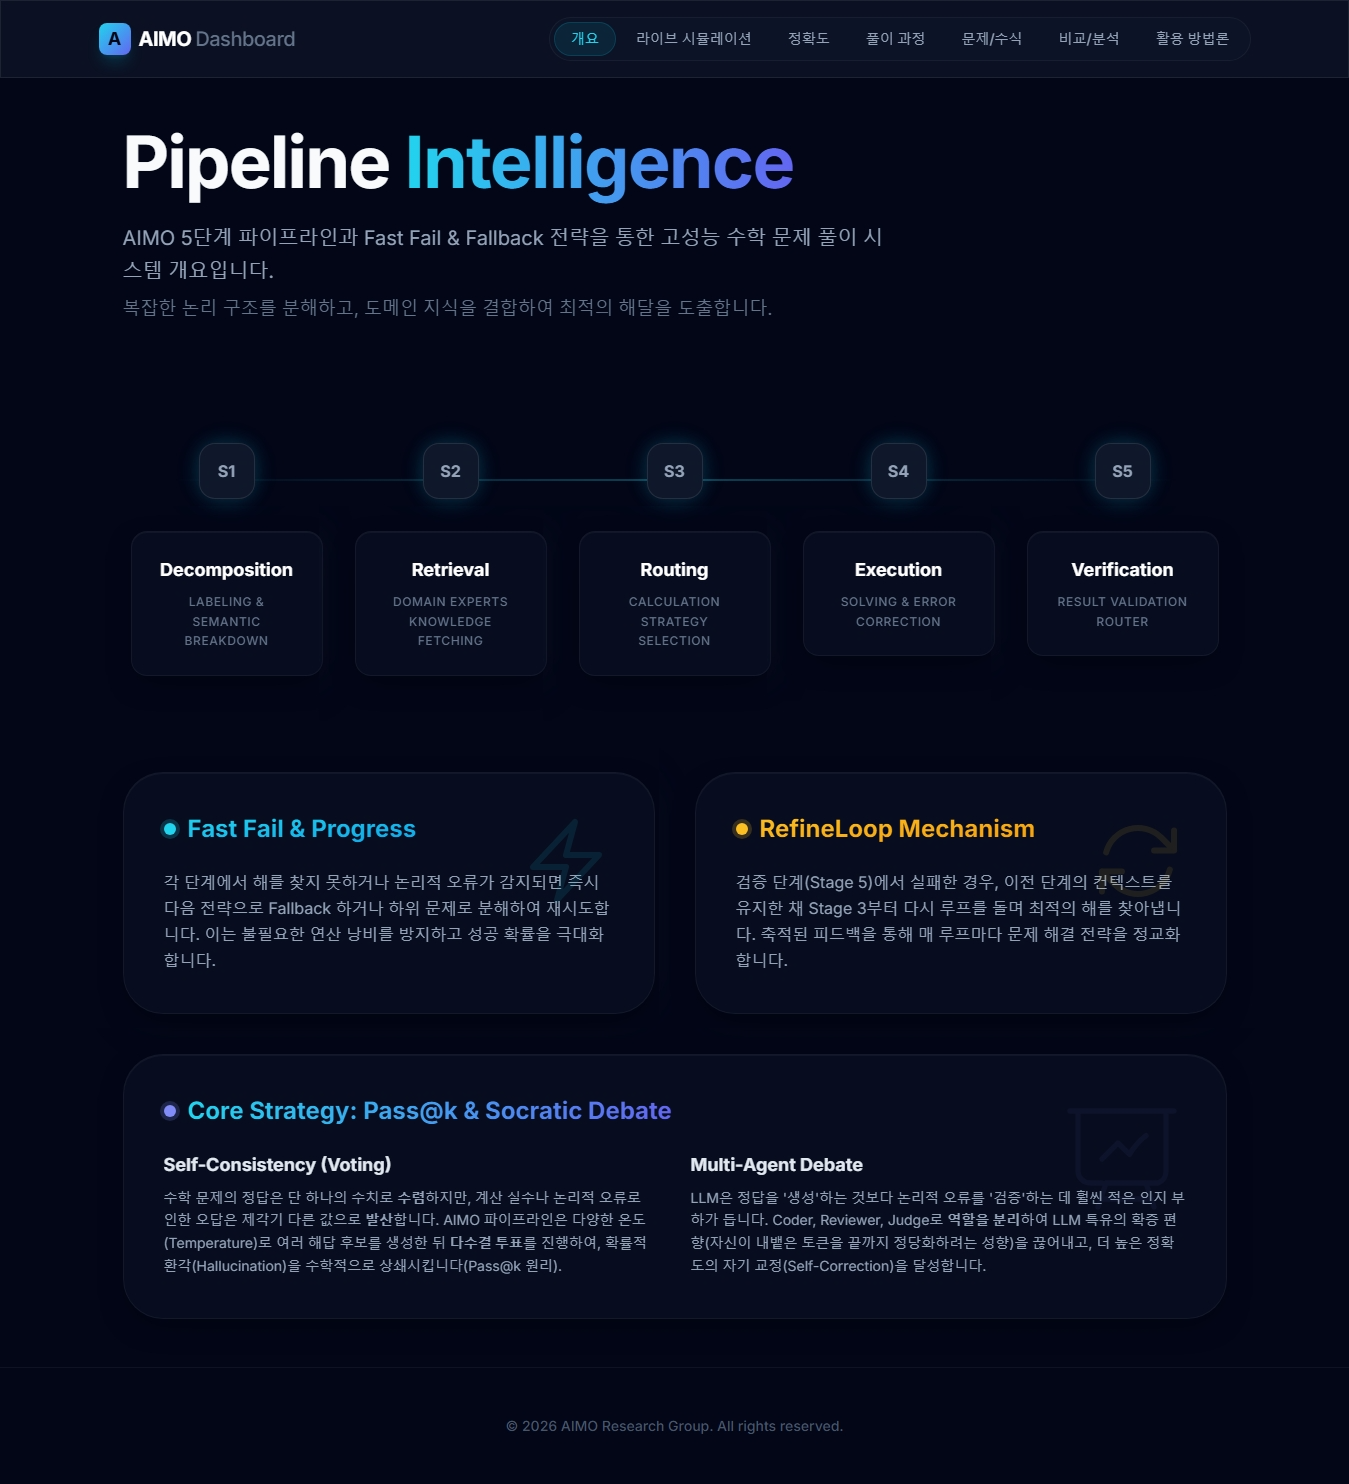
\includegraphics[width=0.95\textwidth]{dashboard_overview.png}
\caption{OMI Glass-box 대시보드 메인 오버뷰(Overview) 화면}
\label{fig:dashboard_overview}
\end{figure}

\subsubsection{XAI (설명 가능한 AI) 및 실전 구동 시나리오}
대시보드를 통해 실제 수학 문제가 풀리는 과정을 다음과 같은 `Glass-box' 시나리오로 구현했습니다.

\vspace{0.5cm}
\noindent\textbf{[User Input]:} ``$100!$ 의 끝에 연속된 0의 개수는 몇 개인가?''

\begin{enumerate}
    \item \textbf{[Stage 1: Labeling] 활성화}
    \begin{itemize}
        \item \textit{UI 표현:} 화면 중앙에 "분석 중..."이라는 스피너가 돌고, 우측 패널에 메타데이터가 JSON 형태로 타이핑됩니다.
        \item \textit{XAI 해석:} "이 문제는 \texttt{정수론(Number Theory)} 도메인이며, 핵심 타겟 변수는 $N=100$ 입니다."
    \end{itemize}
    
    \item \textbf{[Stage 2: Retrieval] 활성화}
    \begin{itemize}
        \item \textit{UI 표현:} 책장 아이콘이 반짝이며, 화면 상단에 '지식 로드 완료' 뱃지가 나타납니다.
        \item \textit{XAI 해석:} "팩토리얼의 0 개수를 구하기 위해 소인수분해 알고리즘과 \texttt{르장드르의 정리(Legendre's formula)} 템플릿을 컨텍스트에 주입했습니다."
    \end{itemize}
    
    \item \textbf{[Stage 3: Router] 활성화}
    \begin{itemize}
        \item \textit{UI 표현:} 3갈래의 파이프 애니메이션 중 가운데의 \textbf{Path B (The Theoretician)} 파이프라인으로 트래픽(빛나는 선)이 흘러갑니다.
        \item \textit{XAI 해석:} "$100!$은 천문학적으로 거대한 수이므로 시뮬레이션(Path A)으로 직접 곱하는 것은 비효율적입니다. 5의 배수를 계산하는 수학 공식을 활용하는 이론적 접근(Path B)을 선택합니다."
    \end{itemize}
    
    \item \textbf{[Stage 4: Execution] 활성화}
    \begin{itemize}
        \item \textit{UI 표현:} 다크 모드의 터미널(가상 IDE) 창이 열리며, AI가 작성하는 파이썬 코드가 한 줄씩 실시간 렌더링됩니다. `Run` 버튼 애니메이션이 작동하고 \texttt{24}라는 결과가 터미널에 출력됩니다.
    \end{itemize}
    
    \item \textbf{[Stage 5: Verification] 활성화}
    \begin{itemize}
        \item \textit{UI 표현:} 방패 모양 아이콘 안에서 체크마크가 표시됩니다.
        \item \textit{XAI 해석:} "작성된 코드의 무결성을 검증하기 위해 $N=10$으로 스케일을 줄여(Scale-Down Test) 실행한 결과 2가 도출되었으며, 이는 10!(=3,628,800)의 실제 0 개수와 일치하므로 논리가 참임을 증명합니다."
    \end{itemize}
\end{enumerate}

이러한 XAI 기반의 시각화 대시보드는 시스템이 도출한 \textbf{정답(24)보다 정답에 도달하는 논리의 흐름(사고의 지도)을 학생들에게 각인시키는 훌륭한 교육적 매개체}로 기능합니다.

그림 \ref{fig:dashboard_live}는 대시보드에서 실제로 이차방정식 문제($x^2 - 5x + 6 = 0$)를 푸는 "Live Solve" 시나리오의 실시간 입출력 화면입니다. 학생들은 자연어 문제의 입력값과 모델이 최종 검증한 수치적 출력값뿐만 아니라, 백엔드에서 시뮬레이션 경로를 타고 흘러가는 오케스트레이터의 5단계 실시간 디버그 로그와 실행 상태 폭포수(Waterfall) 궤적을 직관적으로 확인할 수 있습니다.

\begin{figure}[htbp]
\centering
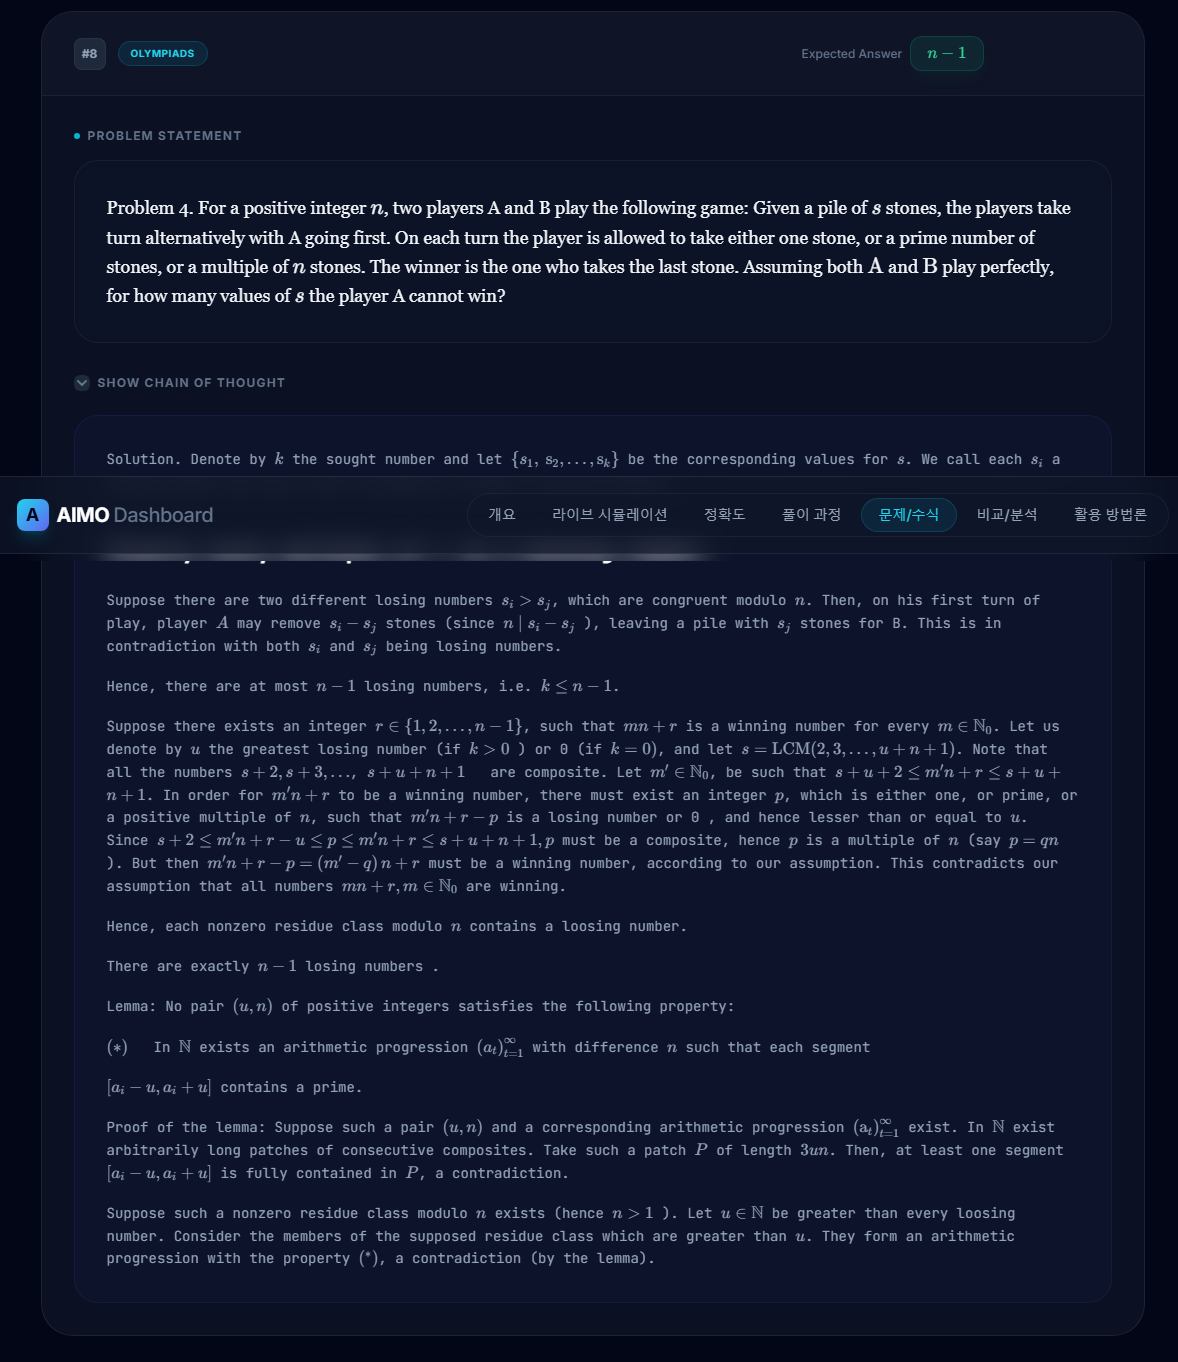
\includegraphics[width=0.95\textwidth]{dashboard_live.png}
\caption{Live Solve 페이지에서의 실제 수학 문제 입출력 및 5단계 추론 트레이스 렌더링}
\label{fig:dashboard_live}
\end{figure}

그림 \ref{fig:dashboard_xai}는 대시보드의 "풀이 과정(XAI Reasoning)" 화면으로, 기하학적 보조선이나 시각 정보가 없는 맹점 상황("눈 없는 AI")에서 수학 문제를 좌표계로 파싱하여 처리하는 단계를 시각화하고, Algebra 및 Combinatorics 등 수학 문제의 난이도별 분포 데이터를 학생들에게 제공하고 있습니다.

\begin{figure}[htbp]
\centering
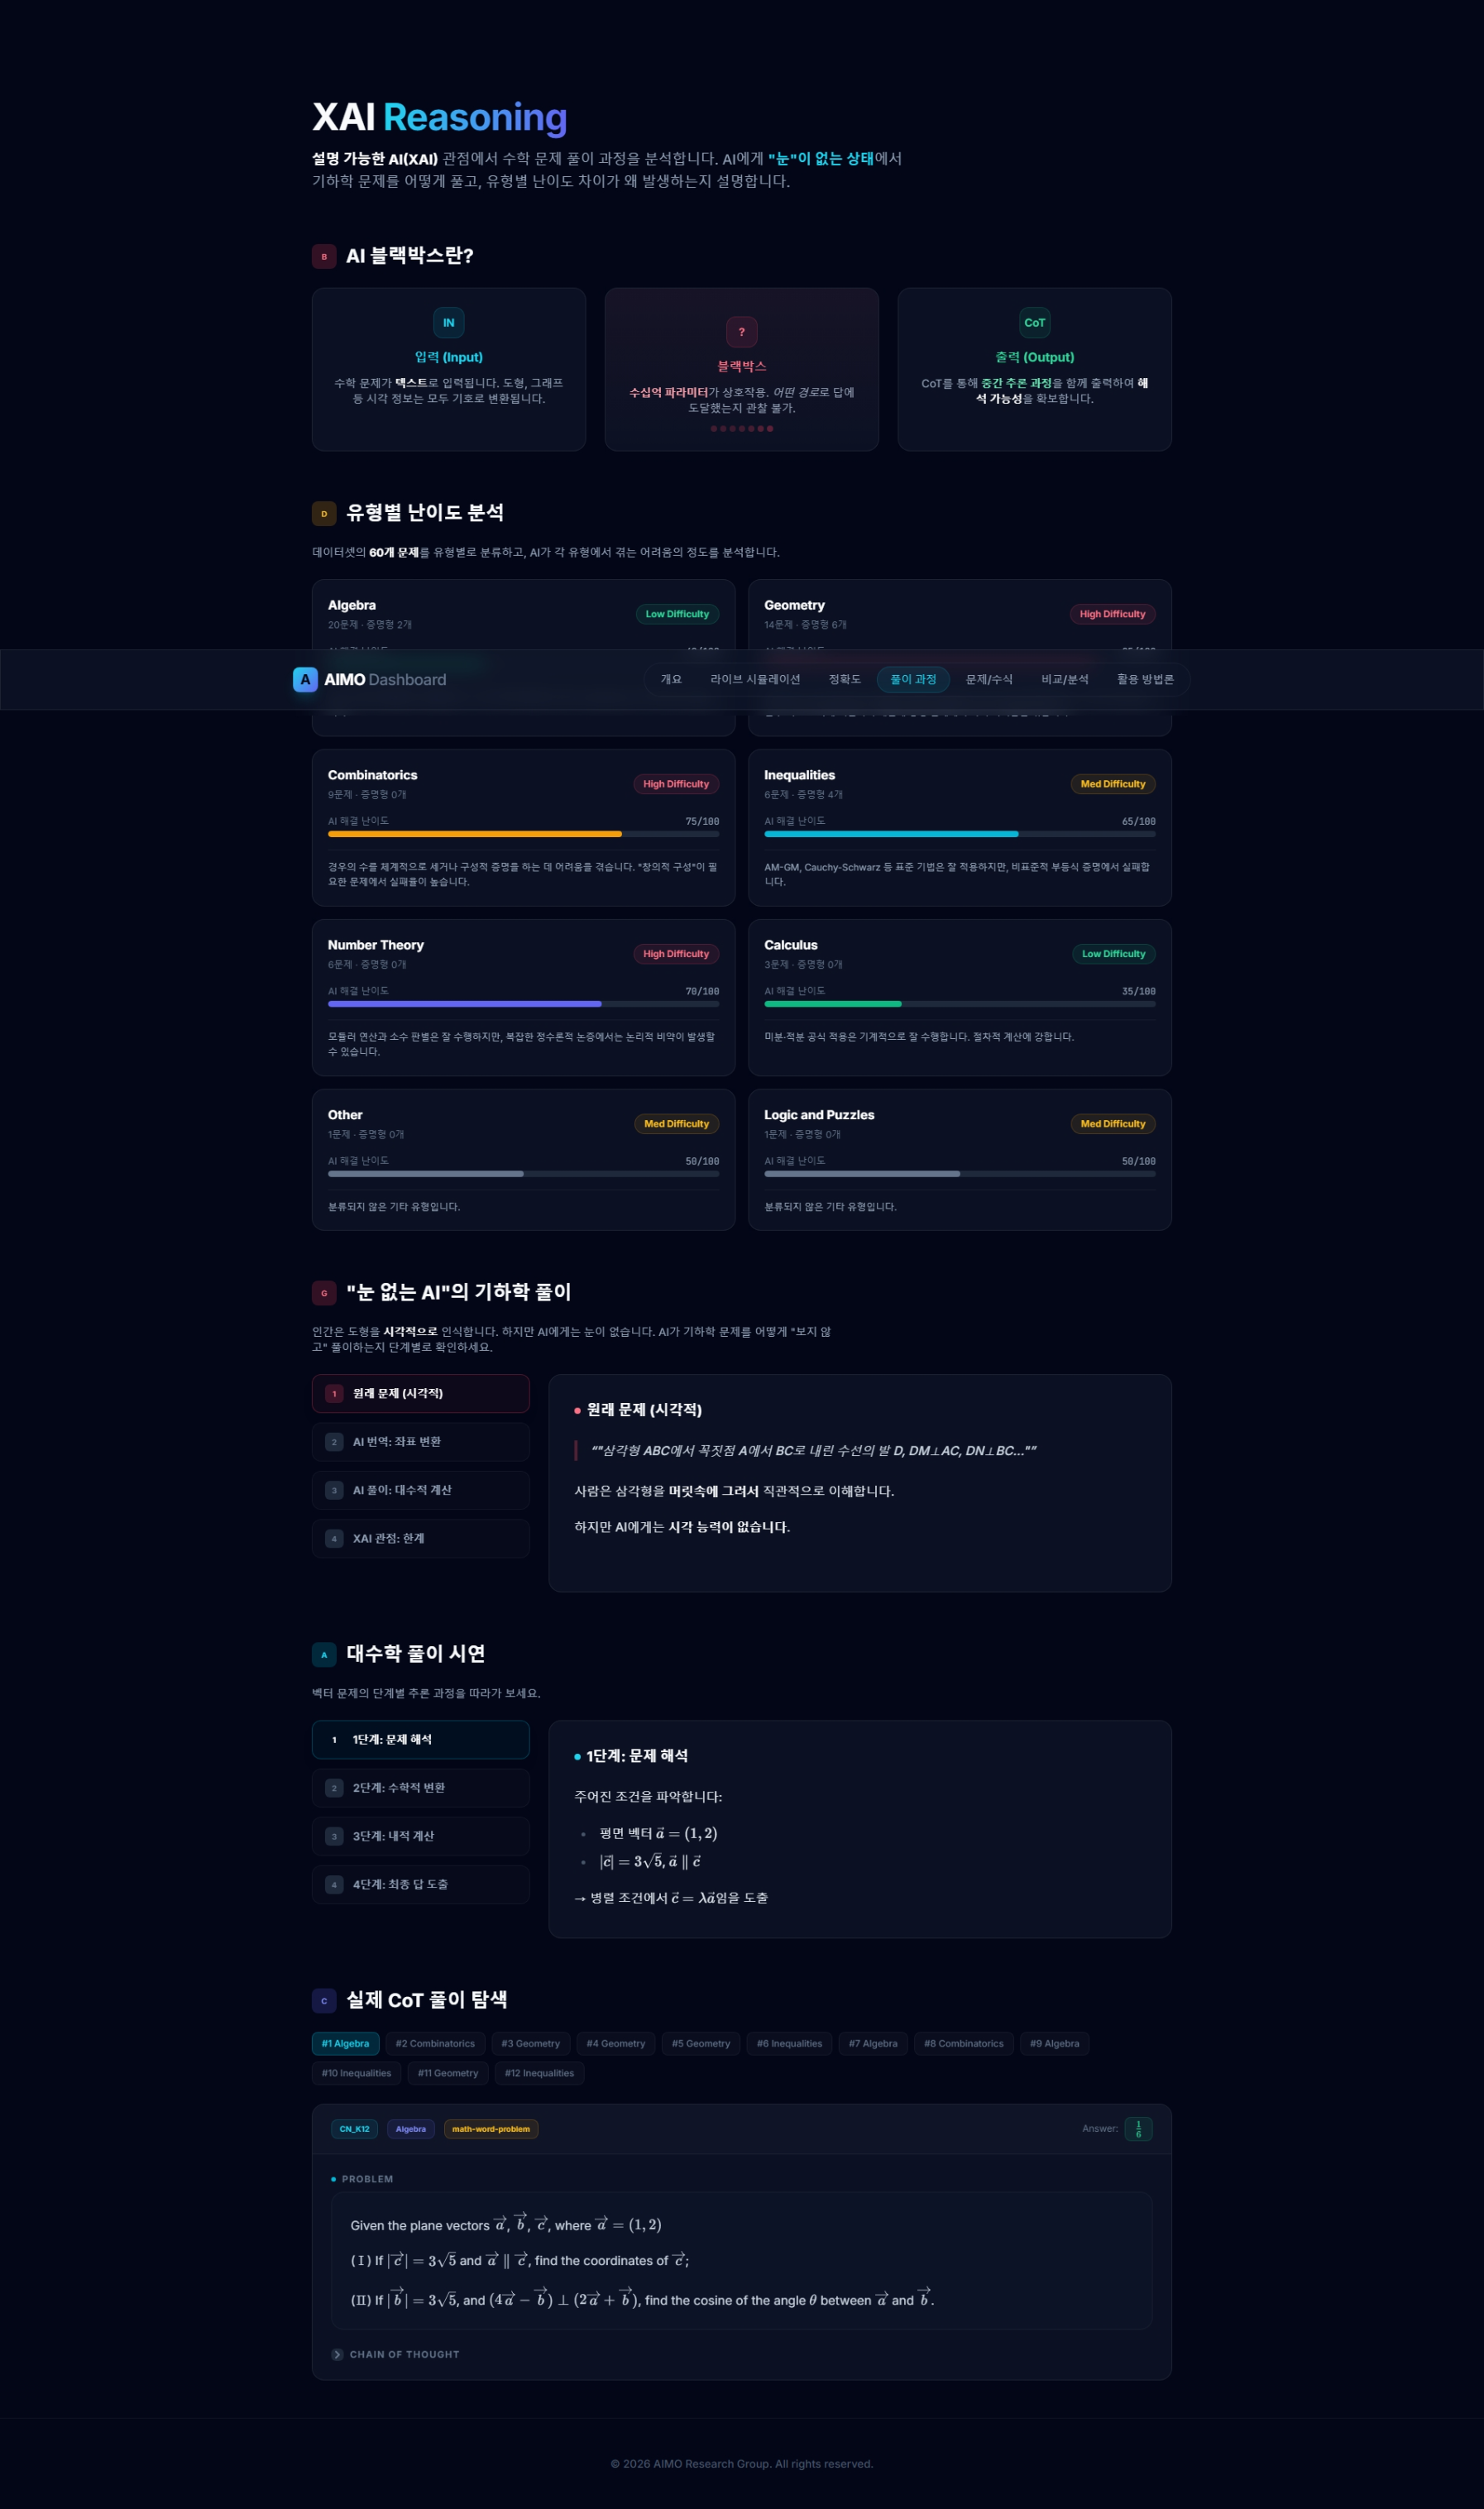
\includegraphics[width=0.95\textwidth]{dashboard_xai.png}
\caption{대시보드의 XAI Reasoning(풀이 과정) 페이지로, 유형별 난이도 분석 및 기하학/대수학 해결 메커니즘을 렌더링}
\label{fig:dashboard_xai}
\end{figure}
